\section{Processing: 45'}

\begin{frame}[fragile]{Simple processing: Goal}
\begin{itemize}
\item Manage gathered data
\item Find relation between them. 
\item Get essential information like standard deviation, 
distribution and linear correlation.
\end{itemize}
\end{frame}

\begin{frame}[fragile]{Simple processing: Agenda}
\begin{itemize}
\item transposing data with zip
\item basic statistics with scipy
\item the importance of standard deviation $\sigma$
\item data distribution and percentiles
\item linear correlation: what's that, when can help
\end{itemize}
\end{frame}

\begin{frame}[fragile]{The Chicken Paradox}
\begin{verse}
"""Statistics says you'll eat a chicken a day. \\
But even if you can't: statistics doesn't fail! \\
Somebody will surely eat two.""" \\
\hfill C. A. Salustri
\end{verse}
\end{frame}

\subsection{Distributions}
\begin{frame}[fragile]{Simple processing: Exercise}
Let's gather some data and try to dismante the chicken paradox
\begin{itemize}
\item Gather 10 seconds of ping output, retrieve a list of RTT
\item Hint: use the sh() function to gather ping output
\item Hint: use zip to put TTL and RTT in two series
\end{itemize}
\end{frame}

\iffalse % solution
def ping_rtt():
    """
       goal: slicing data
       goal: using zip to transpose data
    """
    cmd = "ping -c10 www.google.it"
    if 'win' in sys.platform:
        cmd = "ping -n10 www.google.it"

    ping_output = sh(cmd)
    if 'win' in sys.platform:
        ping_output = [ping_output[6::2] for x in ping_output]
    else:
        ping_output = [ping_output[-4:-1:2] for x in ping_output]
    ttl, rtt = zip(*ping_output)
    return map(float, rtt)
\fi


\begin{frame}[fragile]{Distributions}
A distribution or $\delta$ shows the frequency of events, like 
how many people ate $x$ chickens ;)
\begin{columns}
\column[t]{5cm}
\begin{pythoncode}
#Create a simple $\delta$ with
#    set and dict is easy
distro = {x: rtt.count(x) 
  for x in set(rtt)}
  
# We can even use
from collections \
  import defaultdict
distro = defaultdict(int)
for x in rtt:
    distro[x] += 1
    

\end{pythoncode}
\column[t]{5cm}
Distributions and Mean are both important!
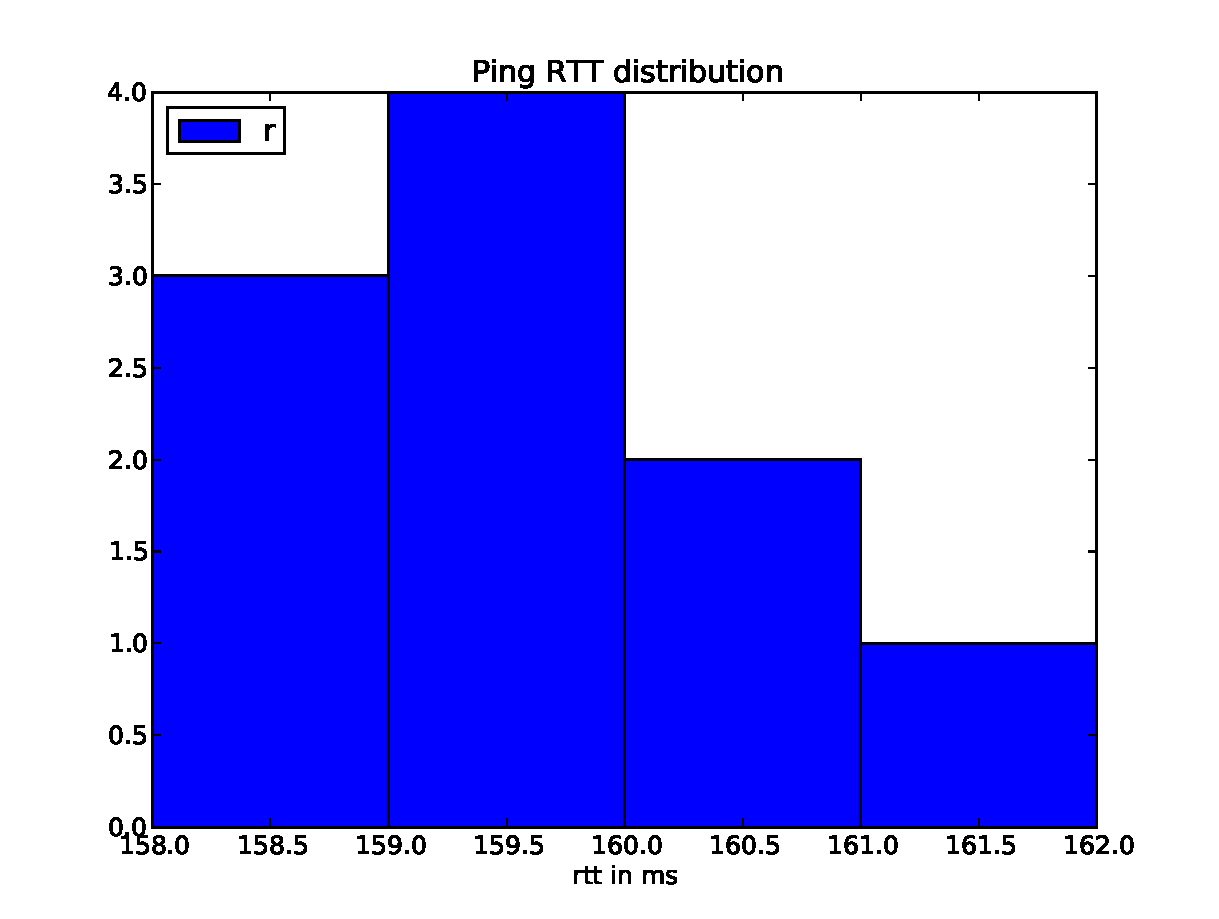
\includegraphics[height=6cm, width=6cm]{ping_distribution.pdf}  
\end{columns}
\end{frame}

\subsection{Deviation}
\begin{frame}[fragile]{Standard Deviation: scipy}
\begin{itemize}
\item Standard deviation or $\sigma$ formula is 
 \\
 $\sigma^{2}(X) := \frac{ \sum(x-\bar{x})^{2} }{n} $
\item $\sigma$ tells if $\delta$ is fair or not, and how much the mean ($\bar{x}$) is representative
\end{itemize}
\begin{pythoncode}
from scipy import std, mean
fair = [1, 1] # chickens
unfair = [0, 2] # chickens
assert mean(fair) == mean(unfair)

# Use standard deviation!
std(fair) # 0
std(unfair) # 1
\end{pythoncode}
\end{frame}


\begin{frame}[fragile]{Simple processing: scipy}
Check your computed values vs the $\sigma$ returned by ping 
(didn't you notice ping returned it?) 
\begin{pythoncode}
def ping_stats():
    """
       goal: remember to convert to numeric / float
       goal: use scipy
       goal: check stdev
    """
    from scipy import std, mean # max,min are builtin
    rtt = ping_rtt()
    fmt_s = 'stdev: {}, mean: {}, min: {}, max: {}'
    rtt_std, rtt_mean = std(rtt), mean(ping_rtt)
    rtt_max, rtt_min = max(rtt), min(ping_rtt)
    print(fmt_s.format(rtt_std, rtt_mean, rtt_max, rtt_min))
\end{pythoncode}
\end{frame}

\begin{frame}[fragile]{Time Distributions: Exercise}
\begin{itemize}
\item Parse the provided maillog in ipython using its magic and get a 4-hourly email $\delta$
\item Expected output: 
\begin{pythoncode}
time_d = {  # mail sent between
    0: xxx  #  00:00 - 03:59
    4: xxx  #  04:00 - 07:59
    ...
    }
\end{pythoncode}
\end{itemize}
\end{frame}
 
\iftrue
\begin{frame}[fragile]{Time Distributions: Exercise Solution}
\begin{pythoncode}
# deliveder emails are like the following
line = "May 14 16:00:04 rpolli postfix/qmgr[11922]: 4AD0C934DA: removed"
def get_slot(ts):
    n = int(ts[:2])
    return n - (n%4)
    
# get the interesting lines
ret = !bzgrep removed maillog
# find the timestamp
ts = ret.fields(2) # 3rd column
hours = [ get_slot(ts)  for x in ts ]
time_d = {x:count(x) for x in set(hours)}
\end{pythoncode}
\end{frame}

\fi 

\begin{frame}[fragile]{Size Distributions: Exercise}
\begin{itemize}
\item Parse the provided maillog file and get a size $\delta$
\item Expected output: 
\begin{pythoncode}
size_d = {  # mail size between
    0: xxx  #  0 - 100k
    1: xxx  #  100k - 200k
    ...
    }
\end{pythoncode}
\item Use the $\delta$ to find size\_mean and size\_sigma
\end{itemize}
\end{frame}



\begin{frame}[fragile]{Simulating data with $\sigma$ and $\bar{x}$}
We can use  mean and a stdev to simulate data using the gaussian distribution.
This is obviously \emph{just a starting point}.
\begin{pythoncode}
from random import gauss
# In a mail load generator script we can simulate a
mail_size = int(gauss(mean, sigma_s))

# and use time_d to simulate the load during the day
from time import localtime
hour = localtime().tm_hour
hour = hour - (hour % 4)
mail_per_minute = time_d[hour] / (4 * 60)
\end{pythoncode}
\end{frame}

\subsection{Correlation}
\begin{frame}[fragile]{Linear Correlation}
T
\begin{pythoncode}
from random import gauss
# In a mail load generator script we can simulate a
mail_size = int(gauss(mean, sigma_s))
# and use time_d to simulate the load during the day

\end{pythoncode}
\end{frame}


def netfishing_correlation():
    from itertools import combinations
    from scipy.stats.stats import pearsonr
    table = {
        'cpu_percent': [10, 23, 55, ...]
        'iops': [2132, 3212, 3942, ...]
        'netio': [1.32e+9, 1.45e+9, ...]
    }
    for k1, k2 in combinations(table, 2):
        r_coeff, probability = pearsonr(table[k1], table[k2])
        print("linear correlation between {} and {} is {}".format(
            k1, k2, r_coeff))
rpolli@rpolli:~/babel/corso_python/python-course/python-for-sysadmin$ 




\begin{frame}[fragile]{Simple processing: Goal}
\begin{itemize}
\item A more flexible script is 02\_ nosetests\_ full.py 
which uses a Test class
\begin{minted}[mathescape]{python}
class Test(object):
    ...
    # Using a Test class...
    def setup(self): 
        print("is_run_before_every_test")

    def teardown(self): # and the same for teardown
        # After every test, eg truncate a table
        print("after_every_test")

    # each test can use the prepared environment
    def test_a(self): 
        assert os.path.isfile("/tmp/test2.out")
 
\end{minted}
\end{itemize}
\end{frame}
